%Créé par Claudine Allen en collaboration avec Jean-Raphaël Carrier
%(Élimination du labo de résistivité des matériaux (IV) à la fin de l'ère JRC + regroupement des labos VI & VII en début de pandémie COVID-19 => renumérotation XI -> IX maintenant)
%Dernière modification JRC: 13 janvier 2014
%Dernière modification CA: 29 novembre 2022
%********************
%ToDo:
% - Essayer de ramener le travail de rétroingénierie sur le système de mesure de l'accélération gravitationnelle en ayant déjà introduit le calcul du temps avec oscillateurs à l'atelier précédent. Je pense diviser le circuit en 3 blocs délimités par des pointillés qui matchent un peu les autres sections du protocole DIY, en partant par la fin : Intro aux circuits logiques rétroactifs -> avec les comparateurs de début de circuit + bascule asynchrone ; Conception du voltmètre -> avec évaluer le résultat d'accélération gravitationnelle à partir de l'oscillateur + compteur (pas de lien conceptuel dans ce cas, juste pcq plus facile/court pour aller avec le voltmètre plus long) ; Construction de portes logiques -> avec les portes NOR ainsi que AND. Il y a deux hics dans tout ça: 1) difficile d'expliquer les portes NOR, AND sans l'info des autres équipes de bascule & oscillateur ; 2) c'est que c'est trop long/redondant de tout le faire en préparation... devrait être fait juste au labo, voir comment exclure de la préparation.
% - Tester le circuit astable avec l'oscillateur de porte NON-OU et rajouter si ça fait encore des attracteurs étrange en simulation... j'en doute. Pourrait aller avec les oscillateurs de l'atelier précédent en remplaçant l'oscillateur à rétroaction qui bouette?
% - Raccourcir en combinant les sections de préparation et déroulement de l'atelier vu que ça répète le début du lab 7 (à recopier au cours 6 aussi). Réviser et ramener les anciens objectifs en renommant "Thématique et objectifs" en voyant si ça ne serait pas mieux de renommer les sous-objectifs en "but à atteindre ou qqch du genre.

\RequirePackage[l2tabu, orthodox]{nag} %Check for obsolete commands
\documentclass[canadien,12pt,oneside,letterpaper]{article}
%
%-----------------------------------------------------
%Loading packages
%
\usepackage[utf8]{inputenc}
\usepackage[T1]{fontenc}
\usepackage[canadien]{babel}
\usepackage{lmodern}
\usepackage{textcomp}
\usepackage{amsmath,amssymb}
\usepackage{siunitx}
\usepackage{xcolor}
\usepackage[colorlinks=true,allcolors=blue]{hyperref}
\usepackage[all]{hypcap}
\usepackage{graphicx}
\usepackage{float}
\usepackage[oldvoltagedirection,americanvoltages,americancurrents,siunitx]{circuitikz}
\usetikzlibrary{babel}
\usepackage{caption}
\usepackage[letterpaper,headheight=15pt]{geometry}
\usepackage{fancyhdr}
\usepackage{setspace}
%
%----------------------------------------------------
%Other configurations and layout
%
\sisetup{separate-uncertainty}
\captionsetup{font=small,labelfont=bf,margin=0.1\textwidth}
\pagestyle{fancy}
\fancyhf{}
\lhead{\textsl{GPH-2006/PHY-2002~---~Atelier~IX}}
\rhead{\textsl{Page \thepage}}
\setcounter{secnumdepth}{0}
\setlength{\parskip}{1.5ex plus0.5ex minus0.2ex}
%\onehalfspacing
\interfootnotelinepenalty=10000 %To avoid footnotes spreading on several pages.
%
%---------------------------------------------------
%
\title{\textbf{Atelier IX}\\Portes \& circuits logiques\thanks{Auteurs: Claudine Allen, Jean-Raphaël Carrier, Denis Panneton, Daniel Bouffard-Landry \& Jérémie Guilbert.}}
\renewcommand\footnotemark{}
\date{}

\begin{document}

\maketitle \vspace{-17ex}

%\section{Objectif}
%
% La dernière fonction de circuits électroniques, mais non la moindre, abordée dans ce cours est le calcul informatique. La fonction d’interrupteur ouvert/fermé du transistor est la clef pour obtenir deux niveaux discrets en tension et ainsi générer un signal numérique binaire permettant des opérations logiques (algèbre de Boole). L’étudiant.e réalisera donc des circuits de portes logiques NON-OU et OU à partir de transistors. En plus de ces opérations logiques, l’ordinateur doit aussi se rappeler rapidement des états binaires entre chaque opération. On introduit alors la rétroaction entre portes logiques, ici en circuits intégrés, pour obtenir une mémoire volatile très rapide d’accès avec une bascule asynchrone SR. Il s’agit d’une mémoire vive (\textit{static random-access memory}, SRAM) de l’ordinateur qui se perd lorsque l’alimentation est coupée, à l’opposé des mémoires de stockage non volatil de l’information binaire. 


% Au lieu de compléter le cours en complexifiant les circuits logiques réalisés à partir d’un schéma, ce laboratoire tentera plutôt d’aider l’étudiant.e à intégrer des connaissances tout en s’exerçant au raisonnement inductif. Concrètement, l’étudiant.e fera la rétro-ingénierie d’un circuit automatisant la mesure du temps de chute d’une masse avec une emphase sur le conditionnement du signal: cette fonction requiert souvent la conception et fabrication de circuits en recherche expérimentale. On bouclera finalement le cours en revenant à la conversion analogique-numérique avec la conception d’un voltmètre à trois niveaux discrets.


% Les travaux effectués aborderont les objectifs d’ensemble 1, 2, 3, 5, 6, 7, 11 et 12 du plan de cours.

\section{Lecture préparatoire}
\vspace{-2.5ex}
\begin{itemize}
\item complément \textit{Introduction aux signaux numériques}
\end{itemize}


% \section{Matériel}

% La réalisation de ce laboratoire requiert l'utilisation de:
% \begin{itemize}
% \item un bloc d'alimentation;
% \item un oscilloscope;
% \item deux résistances de chacune de ces valeurs : 270~$\Omega$, 560~$\Omega$ et 1~k$\Omega$;
% \item une porte NON;
% \item deux diodes électroluminescentes (DEL);
% \item deux portes NON-OU;
% \item trois transistors;
% \item autres composants, selon votre concept de voltmètre;
% \item une plaquette de montage;
% \item un circuit déjà tout monté pour chronométrer la chute d'une bille (partie~1).
% \end{itemize}


% \section{Manipulations}

\setlength{\parskip}{1ex plus 0.5ex minus 0.2ex}

% \section{Préparation}
% Avant de se présenter à la séance de laboratoire, chaque étudiant.e doit:
% \begin{itemize}
% \item lire le complément \textit{Introduction aux signaux numériques};
% \item lire le protocole de ce laboratoire;
% \item débuter, avec un schéma, la conception d'un circuit simple de conversion analogique-numérique en base 1. Ce circuit sera en fait un embryon de voltmètre que vous devrez construire à partir d'une source d'alimentation DC (ou deux au maximum), de la fonction comparateur d'ampli-ops, de résistances et de diodes électroluminescentes (DEL). Ces dernières afficheront la valeur d'un signal de tension dans le système numérotation unaire. Plus précisément, \textbf{aucune} DEL ne doit s'allumer lorsque la tension est inférieure à 1~V, \textbf{une} DEL doit s'allumer lorsque la tension fournie est supérieure à 1~V et \textbf{deux} DEL doivent s'allumer lorsque la tension devient supérieure à 2~V.
% \end{itemize}

\vspace{-3ex}
\section{Préparation}
\vspace{-1.5ex}
\setlength{\parskip}{1ex plus 0.5ex minus 0.2ex}
Les ateliers se rapprochent d'un mode de travail expérimental plus professionnel, car vous devez vous-même préparer votre propre protocole avant d'arriver au laboratoire afin d'atteindre chaque sous-objectif énoncé ci-dessous. Ces sous-objectifs sont généralement accompagnés d'une figure de circuits, mais il y a toutefois progression vers une conception de plus en plus libre où vous devrez proposer vos propres design de circuits. Pour vous assister dans cette rédaction de protocole, les compléments en lecture préparatoire ci-dessus détaillent la théorie et les modèles pour comprendre le fonctionnement des circuits et les analyser expérimentalement. Concrètement dans votre cahier de recherche avec votre coéquipier.ère, écrivez des manipulations et des analyses à faire pour chaque sous-objectif afin de les mettre en commun en plus grand groupe lors de votre arrivée à la séance de laboratoire. 

\vspace{-3ex}
\section{Déroulement de l’atelier}
\vspace{-1.5ex}
Lors de la séance de laboratoire de 2h à la date spécifiée dans la section \texttt{Contenu et activités} sur le site de cours, nous nous diviserons en grands groupes, chacun animé par un membre de l’équipe d’enseignement. Une partie des sous-objectifs et circuits sera attribuée à chaque groupe dans le but d'en faire une présentation orale éducative de 5~minutes pour le reste de la classe à la fin de la séance. La méthodologie de travail en groupe vous appartient alors entièrement pour réussir la meilleure présentation possible qui sera évaluée sur une base ordinale tel qu'expliqué dans la partie synchrone du cours~6.

Nous recommandons de commencer la séance en délibérant sur l'optimisation des manipulations expérimentales et des analyses proposées dans vos cahiers de recherche respectifs avec l'assistance du membre de l'équipe d'enseignement et il vous faudra ensuite répartir les tâches dans votre groupe. Des exemples de tâches possibles sont la planification et l'organisation, la conception, la simulation, la réalisation expérimentale, la mesure, l'analyse, la communication, etc. et il peut bien sûr y avoir de la redondance pour vérifier l'exactitude des résultats de mesure et d'analyse. Notez que la fin de la section \texttt{Matériel didactique} sur le site de cours propose différents choix de logiciels et d'applications pour vous assister dans les tâches de conception et de simulation.

%La dernière activité de la séance sera de vous rendre sur le site Web du cours dans la section \texttt{Évaluations et résultats} pour l'atelier concerné et y évaluer vos pairs sur leur contribution respective au travail du groupe.

% \subsection{Partie 1-Mesure automatisée de l'accélération gravitationnelle}

% Cette partie du laboratoire fonctionne un peu en inverse pour développer des aptitudes de rétroingénierie: le montage est déjà fait et vous devez déduire son fonctionnement logique. Chaque équipe disposera d'une vingtaine de minutes avec le montage, veuillez vous adresser à votre équipe d'enseignement pour coordonner l'accès. L'expérience sera consignée dans un seul et même cahier de laboratoire pour toute la classe. Ce cahier pourra alors assumer sa fonction 
% tour de rôle partir des notes des précédent


% Ce montage sert à mesurer l'accélération gravitationnelle à partir de la chute d'une bille. En fait, il compte le nombre d'oscillations envoyées par un oscillateur entre les événements «de départ» et «d'arrivée», duquel le temps de chute peut être déduit. L'idée générale du montage est illustrée à la figure~\ref{fig:calcul-g}.
% \begin{figure}[h]
% \centering
% 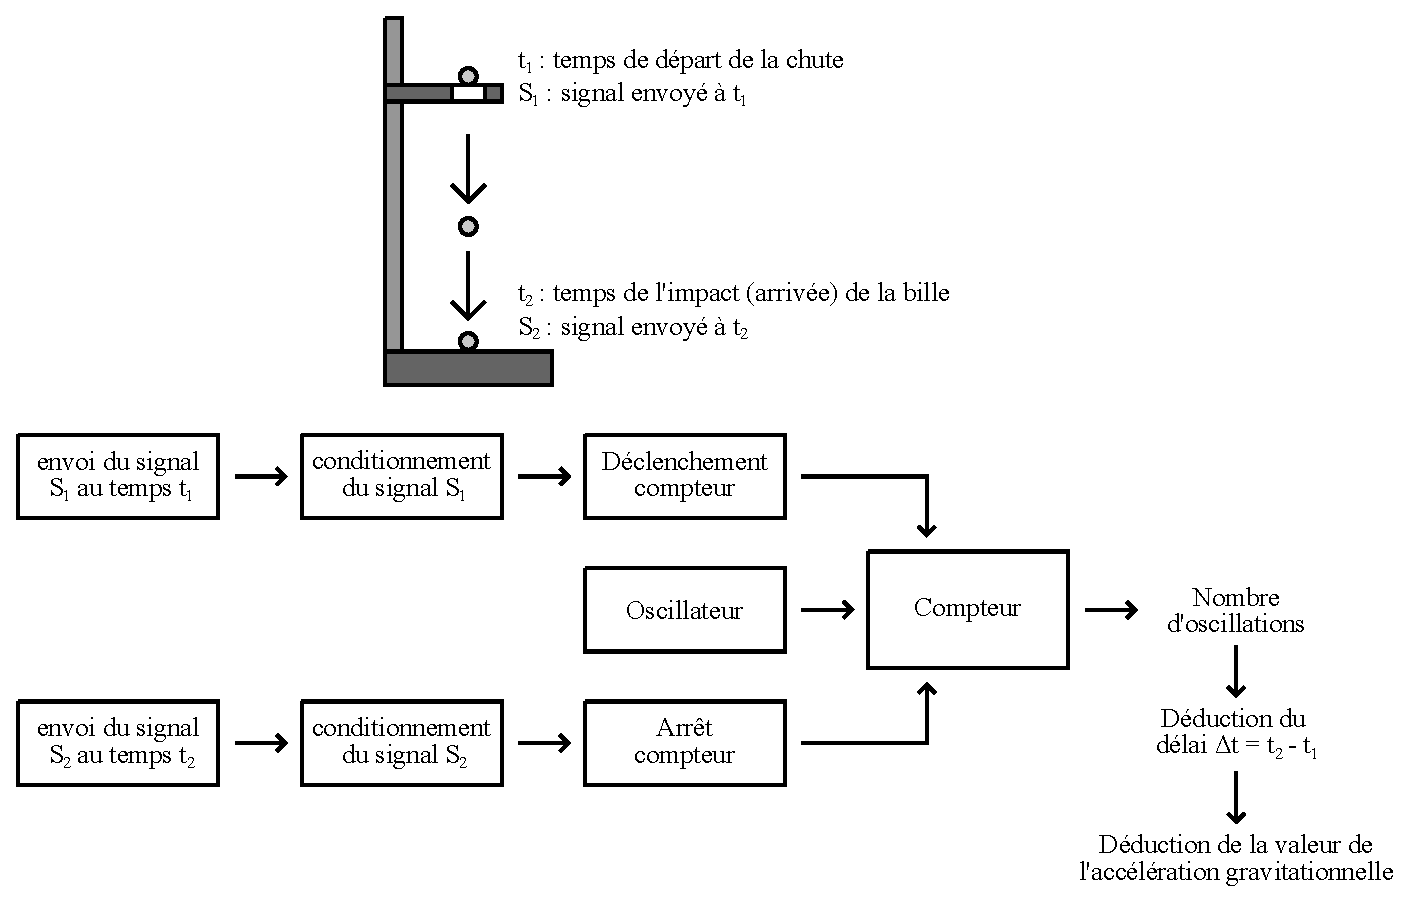
\includegraphics[width=\textwidth]{SchemaFonct-calcul-g}
% \caption{\label{fig:calcul-g}Schéma conceptuel illustrant le fonctionnement général du montage servant à déduire l'accélération gravitationnelle.}
% \end{figure}

% Les manipulations pour cette partie ne sont pas explicitées dans ce protocole. Vous aurez donc à utiliser les fiches techniques des circuits intégrés, un oscilloscope, toute la puissance de votre matière grise, ainsi que l'expérience indéniable que vous avez acquise jusqu'à maintenant, afin de déterminer et de réaliser les manipulations nécessaires. Vos buts sont de comprendre en détail le fonctionnement du circuit et de mesurer l'accélération gravitationnelle en justifiant l'incertitude estimée.

% À la fin du deuxième tour, vous devrez expliquer brièvement comment le circuit parvient à effectuer les fonctions suivantes:
% \begin{enumerate}
%     \item le conditionnement du signal $S_1$ (signal produit par le début de la chute de la bille);
%     \item le conditionnement du signal $S_2$ (signal produit par l'impact de la bille);
%     \item la génération d'un signal à fréquence fixe;
%     \item le déclenchement et l'arrêt du compteur.
% \end{enumerate}

% Complétez l'expérience en écrivant au tableau votre résultat de mesure d'accélération gravitationnelle pour bâtir une distribution statistique avec vos collègues.

\subsection{Construction de portes logiques}

%a) Montez le circuit d'une porte NON-OU (figure~\ref{sch-NOR}) en utilisant les transistors. Appliquez une tension $v_{\mathrm{cc}}$ de 5~V.

 %\noindent\textbf{0\textsuperscript{e} sous-objectif} : En utilisant seulement des puces de portes NON-ET (NAND), concevoir un circuit qui serait équivalent à une porte OU.
 
\begin{figure}[H]
\centering
\begin{circuitikz} \draw
(0,0) node[ground]{} to[Tnpn,n=q1] (0,2) to[short,-*] (5,2) node[right]{$v_{\mathrm{out}}$} to[leDo] (5,0) node[ground]{}
(3,0) node[ground]{} to[Tnpn,n=q2] (3,2) to[R=270~$\Omega$,-o] (3,5) node[above]{$v_{\mathrm{cc}}=5\:\mathrm{V}$}
(-3,1) node[left]{$A$} to[R=560~$\Omega$,o-] (q1.B)
(-3,-2) node[left]{$B$} to[R=560~$\Omega$,o-] (2,-2) to[short] (2,1) to[short] (q2.B); \end{circuitikz}
\caption{\textbf{1\textsuperscript{er} sous-objectif} : À l'aide des entrées A et B en tension ($v_{\mathrm{cc}}\rightarrow$~1, \textit{ground}~$\rightarrow$~0) et de la sortie sur la diode électroluminescente (allumée~$\rightarrow$~1, éteinte~$\rightarrow$~0), consigner la table de vérité et déterminer quelle est la porte logique réalisée par ce circuit. Ajouter ensuite un inverseur à la sortie, constitué d'un transistor et de résistances, pour obtenir une porte OU.}
\label{sch-NOR}
\end{figure}
 
%b) Branchez les entrées $A$ et $B$ soit à l'alimentation, soit à la terre. Faites les quatre possibilités pour construire la table de vérité du circuit afin de vérifier qu'il s'agisse bel et bien d'une porte NON-OU.
%
% c) Rajoutez un inverseur au circuit précédent afin d'obtenir une porte OU (figure~\ref{sch-OR}). Dressez aussi la table de vérité de ce circuit.
% \begin{figure}[h]
% \centering
% \begin{circuitikz} \draw
% (7,1) node[ground]{} to[Tnpn,n=q3] (7,3) to[R=270~$\Omega$,-o] (7,6) node[above]{$v_{\mathrm{cc}}$}
% (0,0) node[ground]{} to[Tnpn,n=q1] (0,2) to[short] (3.5,2) to[R=500~$\Omega$] (q3.B)
% (3,0) node[ground]{} to[Tnpn,n=q2] (3,2) to[R=270~$\Omega$,-o] (3,5) node[above]{$v_{\mathrm{cc}}$}
% (-3,1) node[left]{$A$} to[R=560~$\Omega$,o-] (q1.B)
% (-3,-2) node[left]{$B$} to[R=560~$\Omega$,o-] (2,-2) to[short] (2,1) to[short] (q2.B)
% (7,3) to[short,-*] (9,3) node[right]{$v_{\mathrm{out}}=A+B$} to[leDo] (9,1) node[ground]{}
% ;\end{circuitikz}
% \caption{Circuit interne simplifié d'une porte OU créée en ajoutant une porte NON à la sortie d'une porte NON-OU.}
% \label{sch-OR}
% \end{figure}

\subsection{Conception d'un voltmètre en base 1}

\noindent\textbf{2\textsuperscript{e} sous-objectif} : Réaliser une conversion analogique-numérique en base 1 à l'aide d'un circuit simple. Ce circuit est en fait un embryon de voltmètre à concevoir à partir d'une source d'alimentation DC, de la fonction comparateur d'ampli-ops, de résistances et de diodes électroluminescentes (DEL). Ces dernières afficheront la valeur d'un signal de tension dans le système de numérotation unaire, ce signal étant fourni par un générateur de fonctions ou autre source variable. Plus précisément, \textbf{aucune} DEL ne doit s'allumer lorsque la tension est inférieure à 1~V, \textbf{une} DEL doit s'allumer lorsque la tension fournie est supérieure à 1~V et \textbf{deux} DEL doivent s'allumer lorsque la tension devient supérieure à 2~V.

\subsection{Introduction aux circuits logiques rétroactifs}

% a) Un circuit logique très simple avec rétroaction est constitué uniquement d'un inverseur (porte NON) dont la sortie est retournée à l'entrée. Lorsque l'entrée est \textit{zéro}, la sortie est \textit{un}. Alors l'entrée devient \textit{un} et la sortie \textit{zéro}, et ainsi de suite. On dit que ce circuit est astable, puisqu'il ne possède aucun niveau stable : il s'agit en fait d'un oscillateur. Construisez cet oscillateur (figure~\ref{sch-osc-astable}) et mesurez au mieux, à l'aide de l'oscilloscope, la fréquence des oscillations. Soyez impressionnés de la valeur mesurée.
% \begin{figure}[h]
% \centering
% \begin{circuitikz} \draw
% (0,0) node[not port](not){}
% (not.in) to[short] (-1.5,0) to[short] (-1.5,1) to[short] (1.5,1) to[short] (1.5,0)
% (not.out) to[short] (1.5,0)
% ;\end{circuitikz}
% \caption{\label{sch-osc-astable}Circuit astable créé à partir d'une porte NON.}
% \end{figure}

% b) En plaçant une sonde à l'entrée (canal~1) et une autre à la sortie (canal~2) de l'inverseur, on remarque que ces deux signaux sont reliés malgré leurs fluctuations. Observez l'attracteur qui les relie à l'aide du mode XY de l'oscilloscope. On peut généralement le faire passer d'un cycle limite à un attracteur étrange, et vice versa, en variant l'alimentation de la porte et même en tapant sur la table. Ce système chaotique aura de quoi émerveiller le.la physicien.ne en vous!

%c) Montez le circuit de la bascule asynchrone SR (figure~\ref{sch-RS}) et placez une DEL à chaque sortie. Cette bascule asynchrone est un circuit bistable, puisqu'elle possède deux états stables dits \textit{set} et \textit{reset}.
\begin{figure}[h]
\centering
\begin{circuitikz} \draw
(0,2) node[nor port](norR){}
(norR.in 1) to[short] (-1.5,2.28) node[left]{$R$}
(norR.in 2) to[short] (-2.5,1.72) to[short] (-2.5,-1) to[short] (0.5,-1) to[short] (0.5,0)
(norR.out) to[short] (1,2) node[right]{$Q$}
(0,0) node[nor port](norS){}
(norS.in 1) to[short] (-1.5,0.28) to[short] (-1.5,0.5) to[short] (0.5,1.75) to[short] (0.5,2)
(norS.in 2) to[short] (-1.5,-0.28) node[left]{$S$}
(norS.out) to[short] (1,0) node[right]{$\overline{Q}$}
;\end{circuitikz}
\caption{\textbf{3\textsuperscript{e} sous-objectif} : Déterminer comment ce circuit bistable agit comme une bascule asynchrone sur les entrées S et R en tension.}%% modifier pour faire ressortir le comportement de mémoire vive et ajuster le critère correspondant dans ~Trucs pour dépanner.
\label{sch-RS}
\end{figure}

% Jetons un {\oe}il rapide sur le fonctionnement de cette bascule. Tout d'abord, considérons le cas où l'entrée $R$ (\textit{reset}) est à \textit{un} et l'entrée $S$ à \textit{zéro}. Lorsque $R=1$, la sortie $Q$ est nécessairement à \textit{zéro}, comme nous l'indique la table de vérité de la porte NON-OU. Ceci implique aussi que les entrées de l'autre porte NON-OU (celle du bas) sont à \textit{zéro}, donc $\overline{Q}=1$ et la DEL s'allume. Puis, si $R$ est mis à \textit{zéro}, les sorties $Q$ et $\overline{Q}$ vont conserver leur état, c'est-à-dire $Q=0$ et $\overline{Q}=1$.

% Considérons maintenant le cas où l'entrée $S$ (\textit{set}) est à \textit{un} et l'entrée $R$ est à \textit{zéro}. Lorsque $S=1$, la sortie $\overline{Q}$ est automatiquement à \textit{zéro}, ce qui implique que la sortie $Q$ devient \textit{un} et la DEL s'allume. Si de là on retourne à l'état $S=R=0$, l'état des sorties va à nouveau être conservé : elles vont donc être $Q=1$ et $\overline{Q}=0$. Ainsi, l'état des sorties lorsque $S=R=0$ ne dépend pas uniquement de l'état présent des entrées, mais aussi de l'état précédent des entrées.

% Dans tous les cas considérés précédemment et résumés dans la table de vérité~\ref{table-RS}, les deux sorties ont toujours un comportement opposé : elles sont complémentaires. Autre constat : la mémoire de ce circuit est une \textit{mémoire vive}, elle est volatile. Elle sera effacée du moment qu'une des entrées $S$ ou $R$ sera mise à \textit{un}, ou encore lorsque l'alimentation du circuit sera interrompue.

% d) Dressez la table de vérité du circuit en omettant le cas indéfini où $S=R=1$. Vous devriez obtenir la table de vérité illustrée au tableau~\ref{table-RS}. Vérifiez que les sorties de l'état $S=R=0$ dépendent de l'état précédent du circuit.

% e) Investiguez finalement le cas $S=R=1$ qui n'est pas défini comme fonction de la bascule SR. N'hésitez pas à discuter du comportement avec votre magnifique personnel enseignant!

% \begin{table}
% \centering
% \begin{tabular}{|c|c|c|c|c|}
% \cline{1-4}
% \multicolumn{2}{|c|}{\textbf{Entrées}} & \multicolumn{2}{|c|}{\textbf{Sorties}} \\
% \hline
% $\mathbf{S}$ & $\mathbf{R}$ & $\mathbf{Q}$ & $\mathbf{\overline{Q}}$ & \textbf{Commentaires} \\
% \hline
% 0 & 0 & $q$ & $\overline{q}$ & en mémoire \\
% \hline
% 0 & 1 & 0 & 1 & mise à zéro (\textit{reset}) \\
% \hline
% 1 & 0 & 1 & 0 & mise à un (\textit{set}) \\
% \hline
% \end{tabular}
% \caption{\label{table-RS}Table de vérité partielle de la bascule asynchrone SR.}
% \end{table}

%%%%MOT DE LA FIN SUR MICROPROCESSEURS. (ATELIER: DÉFI OSCILLATEUR LC FAIT EN LIVE POUR BONUS, TOUNES D'OSCILLATEURS)

\end{document}

